\section[Problem Statement]{Problem Statement}

\subsection[Statistical Learning]{Statistical Learning}

\begin{frame}{Dimensionality Reduction in Linear Regression}
	We saw in the linear regression chapter that the statistical learning problem becomes \textbf{ill-posed} when the input features of the problem $x \in \mathcal{X}$ are \textbf{linearly dependent}:
	\begin{itemize}
		\item The matrix $\tilde{X}$ does not have full column rank.
		\item The matrix $\tilde{X}^T \tilde{X}$ is not of full rank and is therefore not invertible.
		\item Multiple solutions exist for the system $\tilde{X}^T \tilde{X} \beta = \tilde{X}^T Y$.
	\end{itemize}
\end{frame}

\begin{frame}{Dimensionality Reduction in Statistical Learning}
	\begin{itemize}
		\item \textbf{Strict} linear dependence is thus a fundamental hurdle when solving linear regression problems.
		\pause 
		\item More broadly, feeding \textbf{highly correlated} input features into a statistical learning algorithm is questionable. Indeed, what is the point of forcing our algorithm to learn from \textit{redundant} information? It increases model complexity (thereby increasing variance) for limited practical benefit.
		\pause
		\item \textbf{Principal Component Analysis} provides an elegant solution to this issue by analyzing the \textbf{interdependencies} among the input features of the problem.
	\end{itemize}
\end{frame}

\begin{frame}{An Obvious Solution. Really?}
	\begin{itemize}
		\item We previously observed that if 2 (or more) input features are linearly dependent or highly correlated, one could simply choose \textit{one of them} as the input for our problem.
		\pause
		\item This is correct, but mathematically unsatisfying: \textit{which one} exactly?
		\pause
		\item Principal Component Analysis proposes instead to take a \textbf{linear combination} of these same features.
	\end{itemize}
\end{frame}

\subsection[General Idea of PCA]{General Idea of PCA}

\begin{frame}{Linear Combination of Input Features}
	If the learning problem features an input space $\mathcal{X} \subset \R^p$, a linear combination of the input features $x^{(i)} \in \mathcal{M}_{1,p}(\R)$ for a given observation $i$ is given by:
	\begin{equation*}
		z^{(i)} = u_1 x_1^{(i)} + u_2 x_2^{(i)} + \cdots + u_p x_p^{(i)} = x^{(i)} u
	\end{equation*}
	\pause
	Where $z$ is a \textbf{score} that combines multiple features, and $u \in \mathcal{M}_{p,1}(\R)$. A score vector $Z \in \mathcal{M}_{n,1}(\R)$ can then be computed for the entire dataset $X \in \mathcal{M}_{n,p}(\R)$:
	\begin{equation*}
		Z = X u
	\end{equation*}
\end{frame}

\begin{frame}{Projection of Observations}
	This operation is equivalent to \textbf{projecting} the observations onto a line $D$ directed by the unit vector $u$. The coordinates of the \textbf{projected} points $\hat{X}$ in the basis $\mathcal{B}$ of $\mathcal{X}$ are written as:
	\begin{equation}
		\hat{X} = Z u^T = X u u^T
		\nonumber
	\end{equation}
	\vspace{-0.8cm}
	\pause
	\begin{columns}
		\begin{column}{0.4\textwidth}
			\begin{itemize}
				\item $Z$ is a scalar representing the distance from the origin to the projection along the line $D$.
				\item The \textbf{error} is defined as the vector between the projection on $D$ ($\hat{X}$) and its original point ($X$).
			\end{itemize}
		\end{column}
		\begin{column}{0.6\textwidth}
			\begin{figure}
				\centering
				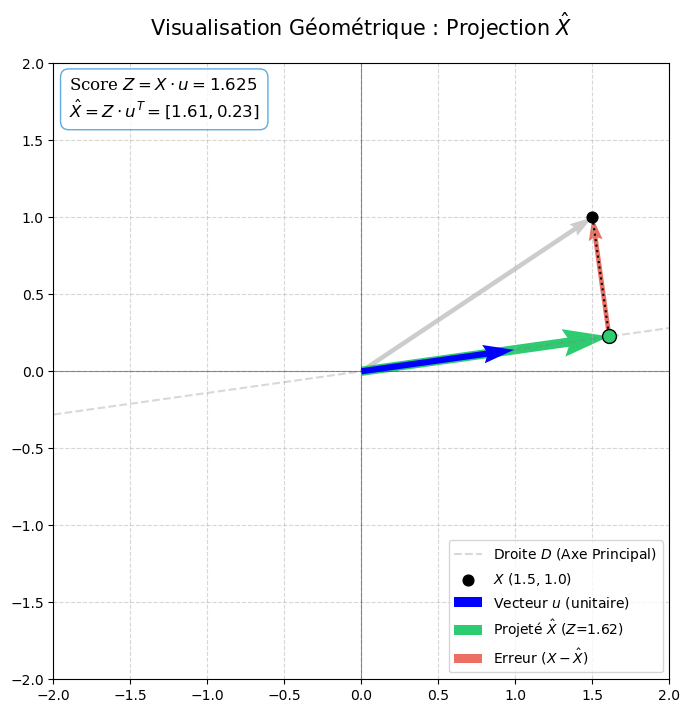
\includegraphics[height=0.75\linewidth]{Images/projection}
				\label{fig:projection}
			\end{figure}
		\end{column}		
	\end{columns}
\end{frame}

\begin{frame}{Principal Component}
	We look for a specific line $D$ and direction vector $u$. The objective of Principal Component Analysis is to choose $u$ such that the variance of the score $Z$ is \textbf{maximized}. This is mathematically equivalent to choosing a line $D$ that minimizes the projection errors $\|X - \hat{X}\|_2^2$. \\
	\vspace{0.5cm}
	\pause
	This line \textbf{must not} be confused with the linear regression line linking the features. For example, with $\mathcal{X} \subset \R^2$:
	\begin{figure}
		\centering
		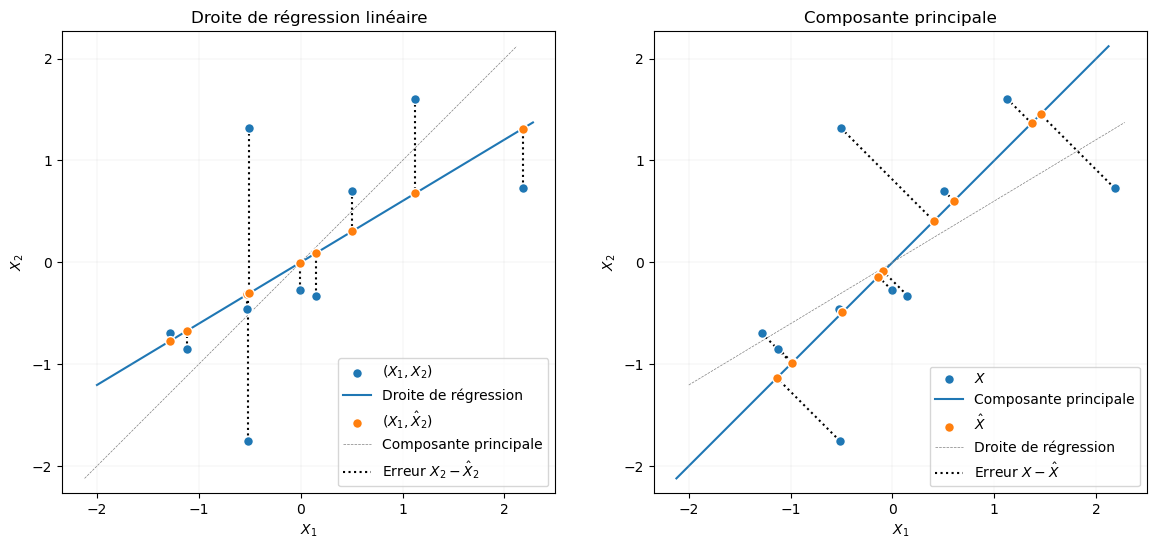
\includegraphics[width=0.85\linewidth]{Images/regression_vs_projection}
		\label{fig:regression_vs_projection}
	\end{figure}
\end{frame}

\subsection[Problem Formulation]{Problem Formulation}

\begin{frame}{Standardized Training Data}
	In Principal Component Analysis, we focus on \textbf{centered} input features $x \in \R^p$ with \textit{similar} variances. One way to ensure centering and variance similarity is to \textbf{standardize} the variables $x_j$ such that across the training data $\mathcal{D} = \{x^{(i)}\}_{i=1}^n$:
	\pause
	\begin{equation}
		\begin{aligned}
			\bar{X}_{\bigdot j} &= \displaystyle \frac{1}{n} \sum_{i=1}^n x_j^{(i)} = 0 \quad \forall j=1, 2, \dots, p \\
			\Varhat{X_{\bigdot j}} &= \displaystyle \frac{1}{n} \sum_{i=1}^n (x_j^{(i)} - \bar{X}_{\bigdot j})^2 = 1 \quad \forall j=1, 2, \dots, p
		\end{aligned}
		\nonumber
	\end{equation}
	\pause
	Where $X_{\bigdot j}$ is the $j$\textsuperscript{th} column of $X$. In the context of PCA, we neglect Bessel's correction, thus working with biased estimators. However, this has no consequence on determining the principal components.
\end{frame}

\begin{frame}{Constrained Optimization for the First Principal Component}
	The first principal component, represented by the line $D_1$ with unit vector $u_1 \in \mathcal{M}_{p,1}(\R)$, is obtained by finding a vector $u_1$ that maximizes the variance of the score $z_1$. We impose a constraint ensuring that $u_1$ remains a unit vector:
	\begin{equation}
		\argmax{u_1 \in \mathcal{M}_{p,1}(\R)} \Varhat{Z_1} \quad \text{s.t.} \quad \|u_1\|_2^2 = 1
		\nonumber
	\end{equation}
	Where:
	\begin{equation}
		Z_1 = X u_1
		\nonumber
	\end{equation}
	We seek the maximum variance of $Z$ in order to summarize the features before explaining the $Y \mid X$ relationship of our statistical learning problem (regression or classification).
\end{frame}

\begin{frame}{Simplifying the Optimization Problem (1/4)}
	Since the training data matrix $X$ is centered:
	\begin{equation}
		\begin{aligned}
			\bar{Z}_1 
			&= \frac{1}{n} \sum_{i=1}^n z_1^{(i)} \\
			&= \frac{1}{n} \sum_{i=1}^n \left(x^{(i)} u_1\right) \\
			&= \left(\frac{1}{n} \sum_{i=1}^n x^{(i)}\right) u_1 \\
			&= \bar{X} u_1 \\
			&= 0
		\end{aligned}
		\nonumber
	\end{equation}
	Where $\bar{X} \in \mathcal{M}_{1,p}(\R)$ represents the mean vector of the columns of $X$. 
\end{frame}

\begin{frame}{Simplifying the Optimization Problem (2/4)}
	\begin{equation}
		\begin{aligned}
			\Varhat{Z_1} 
			&= \frac{1}{n} \sum_{i=1}^n \left(z_1^{(i)} - \bar{Z}_1\right)^2 \\
			&= \frac{1}{n} \sum_{i=1}^n \left(z_1^{(i)}\right)^2 \\
			&= \frac{1}{n} Z_1^T Z_1 \\
			&= \frac{1}{n} (X u_1)^T (X u_1) \\
			&= \frac{1}{n} u_1^T X^T X u_1
		\end{aligned}
		\nonumber
	\end{equation}
\end{frame}

\begin{frame}{Simplifying the Optimization Problem (3/4)}
	The sample covariance matrix computed on the columns of $X$ features the following elements for any $i=1, 2, \dots p$ and $j=1, 2, \dots, p$:
	\begin{equation}
		\begin{aligned}
			\Covhat{X_{\bigdot i}, X_{\bigdot j}} 
			&= \E{\left(X_{\bigdot i} - \E{X_{\bigdot i}}\right)^T \left(X_{\bigdot j} - \E{X_{\bigdot j}}\right)} \\
			&= \E{X_{\bigdot i}^T X_{\bigdot j}} \\
			&= \frac{1}{n} X_{\bigdot i}^T X_{\bigdot j}
		\end{aligned}
		\nonumber
	\end{equation}
	\pause
	We denote $\Sigma$ as the covariance matrix of the columns of $X$:
	\begin{equation}
		\Sigma = \frac{1}{n} X^T X
		\nonumber
	\end{equation}
\end{frame}

\begin{frame}{Simplifying the Optimization Problem (4/4)}
	The variance of $Z_1$ can therefore be written as:
	\begin{equation}
		\begin{aligned}
			\Varhat{Z_1} 
			&= \frac{1}{n} u_1^T X^T X u_1 \\
			&= u_1^T \Sigma u_1
		\end{aligned}
		\nonumber
	\end{equation}	
	\pause
	An alternative way to express the squared Euclidean norm is:
	\begin{equation}
		\|u_1\|_2^2 = u_1^T u_1
		\text{\quad or \quad} \|u_1\|_2^2 = u_1^T u_1
		\nonumber
	\end{equation}
\end{frame}

\begin{frame}{Simplifying the Optimization Problem}
	The initially formulated optimization problem:
	\begin{equation}
		\argmax{u_1 \in \mathcal{M}_{p,1}(\R)} \Varhat{Z_1} \quad \text{s.t.} \quad \|u_1\|_2^2 = 1
		\nonumber
	\end{equation}
	\pause
	can then be simplified to:
	\begin{equation}
		\argmax{u_1 \in \mathcal{M}_{p,1}(\R)} u_1^T \Sigma u_1 \quad \text{s.t.} \quad u_1^T u_1 = 1
		\nonumber
	\end{equation}
\end{frame}

\subsection[Problem Resolution]{Problem Resolution}

\begin{frame}{Resolution Using Lagrange Multipliers}
	This constrained optimization problem can be solved using the method of Lagrange multipliers introduced earlier:
	\begin{equation}
		\argmax{u_1 \in \mathcal{M}_{p,1}(\R)} f(u_1) \quad \text{s.t.} \quad g(u_1) = 0
		\nonumber
	\end{equation}
	With:
	\begin{equation}
		\begin{cases}
			f(u_1) = u_1^T \Sigma u_1 \\
			g(u_1) = u_1^T u_1 - 1
		\end{cases}
		\nonumber
	\end{equation}
	\pause
	The Lagrangian $\mathcal{L}: \R^p \times \R \to \R$ using the Lagrange multiplier $\lambda_1 \in \R$ is given by:
	\begin{equation}
		\mathcal{L}(u_1, \lambda_1) = u_1^T \Sigma u_1 - \lambda_1 \left(u_1^T u_1 - 1\right)
		\nonumber
	\end{equation}
\end{frame}

\begin{frame}{Resolution Using Lagrange Multipliers}
	The stationarity condition of the Lagrangian $\nabla_{u_1} \mathcal{L}(u_1, \lambda_1) = 0$ yields:
	\begin{equation}
		\nabla_{u_1} \mathcal{L}(u_1, \lambda_1) = \nabla_{u_1}\left(u_1^T \Sigma u_1\right) - \lambda_1 \nabla_{u_1}\left(u_1^T u_1\right) = 0
		\nonumber
	\end{equation}
	\pause
	The derivatives of quadratic forms, exploiting the symmetry of $\Sigma$, are as follows:
	\begin{equation}
		\begin{cases}
			\nabla_{u_1}\left(u_1^T \Sigma u_1\right) = 2 \Sigma u_1 \\
			\nabla_{u_1}\left(u_1^T u_1\right) = 2 u_1
		\end{cases}
		\nonumber
	\end{equation}
	\pause
	The stationarity condition therefore becomes:
	\begin{equation}
		\nabla_{u_1} \mathcal{L}(u_1, \lambda_1) = 2 \Sigma u_1 - 2 \lambda_1 u_1 = 0
		\text{\quad or \quad} 2 \Sigma u_1 - 2 \lambda_1 u_1 = 0
		\nonumber
	\end{equation}
	Which simplifies to:
	\begin{equation}
		\Sigma u_1 = \lambda_1 u_1
		\nonumber
	\end{equation}
\end{frame}

\begin{frame}{Resolution Using Lagrange Multipliers}
	We now recognize a fundamental result of linear algebra:
	\begin{itemize}
		\item Solving the PCA optimization problem aligns the first principal component with an \textbf{eigenvector} $u_1$ of the covariance matrix $\Sigma$ of the columns of $X$.
		\pause
		\item The solution Lagrange multiplier $\lambda_1$ is the \textbf{eigenvalue} associated with this eigenvector $u_1$.
		\pause
		\item Since there are $p$ eigenvalues and $p$ associated eigenvectors, we choose the one that maximizes the variance of the score $Z$, which corresponds to the eigenvector associated with the \textbf{largest} eigenvalue.
	\end{itemize}
\end{frame}

\begin{frame}{Finding Subsequent Principal Components}
	\begin{itemize}
		\item Now that we have the \textbf{first} principal component $(u_1, \lambda_1)$, we wish to find the $p-1$ remaining components, starting with the second.
		\pause
		\item We use a similar approach but add a second constraint to our optimization problem: the second principal component must be \textbf{orthogonal} to the first: $u_1^T u_2 = 0$.
		\pause
		\item Seeking an orthogonal direction is justified because the projection error $X - \hat{X}$ is orthogonal to the direction $u_1$. A second orthogonal component thus allows us to \textit{capture} a portion of the variance \textit{missed} during the projection onto the first principal component.
		\pause
		\item And so forth: we will search for a third principal component orthogonal to the first two to capture the remaining variance lost by projecting onto the first two components...
	\end{itemize}
\end{frame}

\begin{frame}{Finding Subsequent Principal Components}
	The optimization problem for the second principal component is then:
	\begin{equation}
		\begin{aligned}
			&\argmax{u_2 \in \mathcal{M}_{p,1}(\R)} u_2^T \Sigma u_2 \\
			&\text{s.t.} 
			\left|
			\begin{array}{ll}
				u_2^T u_2 = 1 & \text{normality condition} \\
				u_1^T u_2 = 0 & \text{orthogonality condition}
			\end{array}
			\right.
		\end{aligned}
		\nonumber
	\end{equation}\\
	\vspace{0.5cm}
	\pause
	The Lagrangian $\mathcal{L}: \R^p \times \R \times \R \to \R$ now introduces two Lagrange multipliers (one for each constraint), $\lambda_2 \in \R$ and $\mu \in \R$:
	\begin{equation}
		\mathcal{L}(u_2, \lambda_2, \mu) = u_2^T \Sigma u_2 - \lambda_2 \left(u_2^T u_2 - 1\right) - \mu \left(u_1^T u_2\right)
		\nonumber
	\end{equation}
\end{frame}

\begin{frame}{Finding Subsequent Principal Components}
	The stationarity condition is written as:
	\begin{equation}
		\nabla_{u_2} \mathcal{L}(u_2, \lambda_2, \mu) = 0 
		\nonumber
	\end{equation}
	\pause
	Which is equivalent to:
	\begin{equation}
		\begin{aligned}
			\nabla_{u_2}\left(u_2^T \Sigma u_2\right) - \lambda_2 \nabla_{u_2}\left(u_2^T u_2\right) - \mu \nabla_{u_2}\left(u_1^T u_2\right) &= 0 \\
			\Rightarrow 2 \Sigma u_2 - 2 \lambda_2 u_2 - \mu u_1 &= 0
		\end{aligned}
		\nonumber
	\end{equation}
	\pause
	Multiplying on the left by $u_1^T$, which is a non-zero vector, yields:
	\begin{equation}
		2 u_1^T \Sigma u_2 - 2 \lambda_2 u_1^T u_2 - \mu u_1^T u_1 = 0
		\nonumber
	\end{equation}
\end{frame}

\begin{frame}{Finding Subsequent Principal Components}
	However, the orthogonality constraint dictates:
	\begin{equation}
		u_1^T u_2 = 0 
		\nonumber
	\end{equation}
	\pause
	Furthermore:
	\begin{equation}
		\begin{aligned}
			u_1^T \Sigma u_2 
			&= \left(\Sigma^T u_1\right)^T u_2 \\
			&= \left(\Sigma u_1\right)^T u_2 \\
			&= \left(\lambda_1 u_1\right)^T u_2 \\
			&= \lambda_1 u_1^T u_2 \\
			&= 0 \quad \quad \text{(orthogonality constraint)}
		\end{aligned}
		\nonumber
	\end{equation}
\end{frame}

\begin{frame}{Finding Subsequent Principal Components}
	The stationarity condition therefore reduces to:
	\begin{equation}
		\mu u_1^T u_1 = 0
		\nonumber
	\end{equation}
	Since $u_1$ is a non-zero vector, it must hold that $\mu = 0$. \\
	\pause
	\vspace{0.5cm}
	The Lagrangian then simplifies to:
	\begin{equation}
		\mathcal{L}(u_2, \lambda_2) = u_2^T \Sigma u_2 - \lambda_2 \left(u_2^T u_2 - 1\right)
		\nonumber
	\end{equation}
	\pause
	It takes \textbf{exactly} the same form as the one used when searching for the first principal component.
\end{frame}

\begin{frame}{Principal Component Analysis}
	\begin{block}{Principal Component Analysis}
		Finding the eigenvalues $\lambda$ and eigenvectors $u$ of the covariance matrix $\Sigma$ computed on the columns of $X \in \mathcal{X}$ allows us to determine all the principal components. The first component is associated with the largest eigenvalue, the second with the next largest, and so on...
		\begin{equation}
			\Sigma u = \lambda u
			\nonumber
		\end{equation}
	\end{block}
\end{frame}